\section{Results}
\subsection{Held-Out Whole-Connectome Tests}
Frozen calibration yielded healthy collision-free survival in 5/6 cases at $-30^\circ$ and 0/6 at $+30^\circ$ (Fig.~\ref{fig:prospective}). The corresponding counts were 4/6 and 0/6 under 25\% deletion; 50\% deletion and readout disabling yielded 0/12 each. On paired negative-bearing seeds, deletion lost one and five healthy survivors, respectively; the positive bearing was already at floor. These are six-cluster conditional observations. For 50\% deletion, matched spike ratios were 0.748/0.845/0.890/1.012 over 200/300/400/500\,ms. Neither deletion condition exceeded twice its paired healthy activity in those windows, despite eight and twelve collisions. Thus this activity limit did not flag these outcomes. It is distinct from the open-loop joint rule.

\begin{figure}[t]
\centering
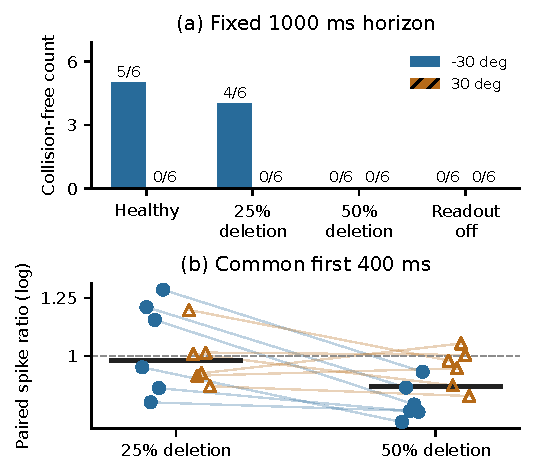
\includegraphics[width=\columnwidth]{figs/prospective_outcomes.pdf}
\caption{First prospective campaign, seeds 6--11. (a) Collision-free counts at 1000\,ms, six seeds per bearing. (b) Every 400\,ms activity pair: circles $-30^\circ$, triangles $+30^\circ$, black median. Thin lines connect the same seed/bearing across deletion doses. Shared seeds are not independent replicates. This activity limit did not distinguish the observed collisions; no predictive detector was fitted.}
\label{fig:prospective}
\end{figure}

\subsection{Controller-by-Fault Comparison}
All 12 first-campaign healthy tests turned $-11.429^\circ$ before the 100\,ms cue while recording zero spikes. Equation~\eqref{eq:steering} produces $-114.286^\circ$/s at zero readout. Readout disabling removes both this offset and the neural trigger, so its comparison alone cannot isolate stimulus-dependent steering.
\begin{table}[t]
\caption{Frozen controller $\times$ fault comparison, seeds 12--17. Six clusters share both bearings and all conditions. L/G: paired healthy-to-fault losses/gains out of 12; healthy survivors at risk are four/six under original/gated laws. Healthy rows reuse preserved records.}
\label{tab:steering}
\centering\small
\setlength{\tabcolsep}{3pt}
\begin{tabular}{llrrrr}
\toprule
Law & Network & $-30^\circ$ & $+30^\circ$ & Total & L/G\\
\midrule
Original & Healthy & 4/6 & 0/6 & 4/12 & ---\\
Original & 25\% deletion & 4/6 & 0/6 & 4/12 & 1/1\\
Original & 50\% deletion & 0/6 & 0/6 & 0/12 & 4/0\\
Pre-cue gate & Healthy & 6/6 & 0/6 & 6/12 & ---\\
Pre-cue gate & 25\% deletion & 3/6 & 0/6 & 3/12 & 3/0\\
Pre-cue gate & 50\% deletion & 0/6 & 0/6 & 0/12 & 6/0\\
\bottomrule\end{tabular}\end{table}

The 72-record matrix directly pairs each fault with its
same-law healthy reference (Table~\ref{tab:steering}). The healthy gate advantage
is two episodes out of 12 (+16.7 percentage points); its six-cluster conditional
range includes zero. Offset-only and no-steering healthy controls triggered
bursts in 11/12 and 12/12 cases but yielded 0/12 survival (Supplementary
Tables~S12--S14). These compare complete feedback laws, which can change sensory
trajectories and trigger timing.

At 25\% deletion, gated-minus-original net task loss was +25.0 percentage points (conditional 95\% range 8.3 to 41.7). At 50\% deletion, gated-minus-original net task loss was +16.7 percentage points (conditional 95\% range 0.0 to 33.3). The 25\% range excludes zero, but only 3 seed clusters have nonzero interactions; a post-hoc symmetric-null sign-flip sensitivity gives $p=0.25$ (Supplementary Section~13). At 50\% deletion, both controllers yield 0/12; their net-loss contrast reflects different healthy baselines. Loss and gain counts are retained separately; a healthy success difference alone is not a fault-tolerance comparison.

Among 48 faulty episodes, 41 collided; none of these collisions was flagged at any tested $c=1.5,2,3,4$ over 200--500\,ms. At 500\,ms, $c=1.5$ instead flagged 2 surviving fault episodes. This activity-only criterion did not distinguish the observed collisions under these settings; it does not establish that spike count is generally uninformative. Supplementary Table~S22 and the threshold CSV report the full sensitivity.


\subsection{Transmission Under Five Perturbation Families}
Healthy command rate is 94.69\,Hz (95\% median CI 94.06--95.42), with first-spike latency 4.05\,ms. Equal-sized random drive yields approximately 8.2\,Hz despite greater activity; the intact target-permuted graph yields zero. This specificity does not isolate a fault-tolerance mechanism.

The supplement supplies every main dose, recorded control damage and selected-dose intervals. F1 at $\sigma=0.50$ retained 99.4\% of median rate, with 10th--90th percentiles 90.40--100.81\,Hz versus healthy 93.96--95.63\,Hz. F3 at 10\% retained 100.4\%. These sampled medians do not establish equivalence.

F2 retained 97.0\%, 98.3\%, 89.2\% and 76.5\% of median command rate at 5\%, 10\%, 25\% and 50\% deletion. The 95\% bootstrap interval for the ratio of median rates at 50\% was 75.1--79.0\%. Latency rose from 4.05 to 5.40\,ms (ratio 1.33, interval 1.25--1.40). All sampled deletion trials passed transmission; a separate 75\,Hz control passed only 10/12 at 50\% deletion. F5 retained 79.8\% or 67.9\% when removing LC4 or LPLC2 outputs; silencing both eliminated transmission. Supplementary plots show all doses and dispersion.

Twelve new 600\,ms runs tested the sensory refractory variant on three paired seeds. Median paired 50\%-deletion retention was 76.3\% at 2.2\,ms versus 79.2\% at zero sensory refractory time. Healthy median rates were 94.8 and 103.1\,Hz. These conditional observations do not establish variant invariance.

\subsection{Historical Hub Records and Activity Scoring}
The historical 1\% F4 condition yielded 119.06\,Hz and 49{,}272.5 median spikes (1.24$\times$ healthy). Cell manifests are missing; reconstructed selection includes protected readout cells, and implementations differ. Historical contrasts cannot be attributed to cell sign alone. The artifact's \path{audit/verified-hubs} contains selector reconstructions, not recovered historical manifests; Supplementary Table~S4 gives recorded damage.

The inhibitory subset had 847{,}476.5 median spikes (21.35$\times$ healthy), failing the activity criterion in 12/12 trials. The random inhibitory expected-contact-mass control had median 50{,}323 spikes, with two extreme trials (327{,}246 and 271{,}058). Individual records and realized damage are supplied.

Across 288 fault/control records, 276 passed transmission and 262 jointly. Twelve extra rejections arose from inhibitory hubs and two from random-mass records (Table~\ref{tab:cohorts}). Excluding targeted hubs left two disagreements among 204 records; the main non-hub sweep had none. Counts were unchanged for $c=1.5,2,3,4$. All 12 healthy reference trials passed, but resubstitution does not estimate held-out false alarms or calibrate the limit.

\begin{table}[t]
\caption{Post-hoc cohort sensitivity, $c=2$. T: transmission; J: joint passes. EIm: composition-matched controls. Rows successively isolate the inhibitory subset, all targeted-hub cohorts, then the main non-hub sweep by removing whole conditions. Remaining disagreements are random-mass trials 3 and 9; mixtures do not estimate population failure probability.}
\label{tab:cohorts}
\centering\small
\setlength{\tabcolsep}{4pt}
\begin{tabular}{lrrrr}
\toprule
Included records & $n$ & T & J & T$-$J\\
\midrule
All faults/controls & 288 & 276 & 262 & 14\\
Exclude inhibitory hubs & 276 & 264 & 262 & 2\\
Exclude F4/HUB/EIm & 204 & 192 & 190 & 2\\
Main F1/F2/F3/F5 & 180 & 168 & 168 & 0\\
\bottomrule
\end{tabular}
\end{table}

\subsection{Legacy Evaluation and Stopping-Time Matching}
Legacy looming used elapsed time and heading canceled from receptive-field bearing. Six threshold-calibration logs duplicate healthy evaluation records; all fault episodes share calibration seeds. Four-bearing/three-seed survival was 10/12 for 25\% deletion, 0/12 for 50\%, 12/12 for full hubs and 6/12 for inhibitory hubs. Eight healthy records stopped during a burst. These are compromised recorded-horizon illustrations, not corrected geometric tests (Supplementary Table~S5).

For legacy 50\% deletion, early collisions shorten fault records relative to healthy references. Matching each pair to $T_*$ changes the median spike ratio from $R_{\mathrm{whole}}=0.382$ to $R_{\mathrm{common}}=0.729$. Fixed 200--500\,ms ratios span 0.723--0.745. This stopping-time mismatch is distinct from the horizon effect below; neither ratio defines an activity budget.

\begin{figure}[t]
\centering
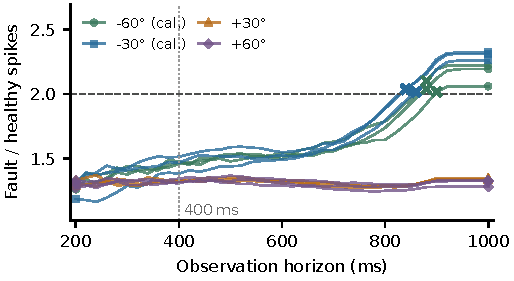
\includegraphics[width=\columnwidth]{figs/late_hubs.pdf}
\caption{Legacy full-hub cumulative activity ratios. Both members of every pair last 1000\,ms. Marker/color encode bearing; three same-bearing traces are shared seeds. Negative bearings are calibration scenarios. Crosses mark first twofold crossings at 840--900\,ms. The first 400\,ms excludes late activity rather than correcting unequal durations.}
\label{fig:demo}
\end{figure}

\subsection{Late Activity Under Equal Durations}
All full-hub and paired healthy records last 1000\,ms, so $R_{\mathrm{whole}}=R_{\mathrm{common}}$ for each pair. No ratio exceeds twofold through 800\,ms. Six first crossings occur at 840--900\,ms, all at $-60^\circ$ or $-30^\circ$ on calibration seeds (Fig.~\ref{fig:demo}). Thus selecting 400\,ms excludes late exceedances; it does not remove unequal exposure. Pooled medians rise from 1.362 at 400\,ms to 1.703 at 1000\,ms. Inhibitory hubs exceed twofold in every pair at all 200--500\,ms windows. Individual trajectories and three-seed sensitivity are supplied; sparse conditional bootstrap ranges do not establish independent reliability.

The privileged geometry rule survives both bearings at 800 and 1000\,ms but collides by 1200\,ms. This establishes bounded task feasibility with identical actuator limits, without a neural resource-cost comparison. The supplement records each seed, termination and generating manifest.
